\section{History}\label{sec:history}

\begin{wrapfigure}{R}{0.3\textwidth}
\centering
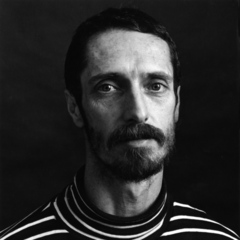
\includegraphics[width=0.25\textwidth]{images/history}
\end{wrapfigure}

CI was developed \textbf{1972} in the US by mainly \textbf{Steve Paxton}, see picture on the right, (along with Nancy Stark Smith, Danny Lepkoff, Lisa Nelson, and others) which was an American dancer, gymnastics and choreographer (and former Aikidoka, someone who practices the Japanese martial art Aikido).
He wanted to explore and push the boundaries to develop this new practice, some sort of ``art-sport''.

For that purpose, he gathered with a group of dancers and athletes to explore the \textbf{extremes of movement} and disorientation, from standing still to falling, rolling, colliding and jumping in the air.
To see for yourself how the first steps were made, have a look at this old recording: \url{https://www.youtube.com/watch?v=9FeSDsmIeHA}

Out of that exploration, a 20-minutes performance piece called ``\textit{Magnesium}'' arose, whereas the first quarter hour was about jumping and bumping, manipulation and clinging.
Only the last 5 minutes the so-called ``Small Dance'' was performed: A form of meditation that is practiced standing, where attention is paid to postural adjustments and micro-weight transfers.

In spring 1972, Steve Paxton invited dancers to work on the form he was evolving, and at the end of this week of residency, the group presented a performance named \textbf{Contact Improvisations}.
The members of the group scattered across the US and started to teach the practice.
It became more smooth, continuous and controlled, yet still avoiding eye and direct hand contact.
Much emphasize was put on the experience of flow, which is more of an aesthetic choice (Nancy Stark Smith), yet the central characteristics preserved.
See chapter \textit{What} for more details on that.

At first, around 1975, it was considered to \textbf{trademark} the term contact improvisation, but this idea was rejected in favor of establishing a forum for communication, which nowadays is the online website \url{https://contactquarterly.com}, which is still co-edited by Nancy Stark Smith herself.
A few years later, 1979, the very first ``Country Jam'' was organized, where 50 people came together to freely exchange and dance, without any structure.
Neither a workshop, conference or seminar.
Co-created being, dancing and living in flux.

\textbf{Europe} was presented with CI first 1873 in Italy, and later Steve Paxton and Lisa Nelson regularly went to the UK and Amsterdam (School for New Dance Development) as the transmission belts for CI in the whole of Europe.
Belgium was visited by Paxton since the 1980s, but apart certain outbreaks of fever in successful jams, it didn't leave any lasting traces among dancers.

\textbf{Jams} were introduced in the mid-1970s, a form of social gatherings as known from jazz jam sessions or milongas in tango.
It's an opportunity to practice freely, where people can meet and negotiate together their dance or observe the practice of their partners.
It's a hybrid between bodily meditation, psycho-kinesthetic therapy, sports training and a dance improvised session.